%====================================================================%
%                  MORIOND.TEX                                       %
%====================================================================%

\documentclass{moriond}

\usepackage{lineno}

% I want to have square brackets
\usepackage[square,numbers]{natbib}

\bibliographystyle{unsrt}    
% for BibTeX - sorted numerical labels by order of
% first citation.

% A useful Journal macro
\def\Journal#1#2#3#4{{#1} {\bf #2}, #3 (#4)}

% Some useful journal names
\def\NCA{\em Nuovo Cimento}
\def\NIM{\em Nucl. Instrum. Methods}
\def\NIMA{{\em Nucl. Instrum. Methods} A}
\def\NPB{{\em Nucl. Phys.} B}
\def\PLB{{\em Phys. Lett.}  B}
\def\PRL{\em Phys. Rev. Lett.}
\def\PRD{{\em Phys. Rev.} D}
\def\ZPC{{\em Z. Phys.} C}

% Some other macros used in the sample text
\def\st{\scriptstyle}
\def\sst{\scriptscriptstyle}
\def\mco{\multicolumn}
\def\epp{\epsilon^{\prime}}
\def\vep{\varepsilon}
\def\ra{\rightarrow}
\def\ppg{\pi^+\pi^-\gamma}
\def\vp{{\bf p}}
\def\ko{K^0}
\def\kb{\bar{K^0}}
\def\al{\alpha}
\def\ab{\bar{\alpha}}
\def\be{\begin{equation}}
\def\ee{\end{equation}}
\def\bea{\begin{eqnarray}}
\def\eea{\end{eqnarray}}
\def\CPbar{\hbox{{\rm CP}\hskip-1.80em{/}}}
%temp replacement due to no font
%%%%%%%%%%%%%%%%%%%%%%%%%%%%%%%%%%%%%%%%%%%%%%%%%%
%                                                %
%    BEGINNING OF TEXT                           %
%                                                %
%%%%%%%%%%%%%%%%%%%%%%%%%%%%%%%%%%%%%%%%%%%%%%%%%%

%\newcommand{\Photo}{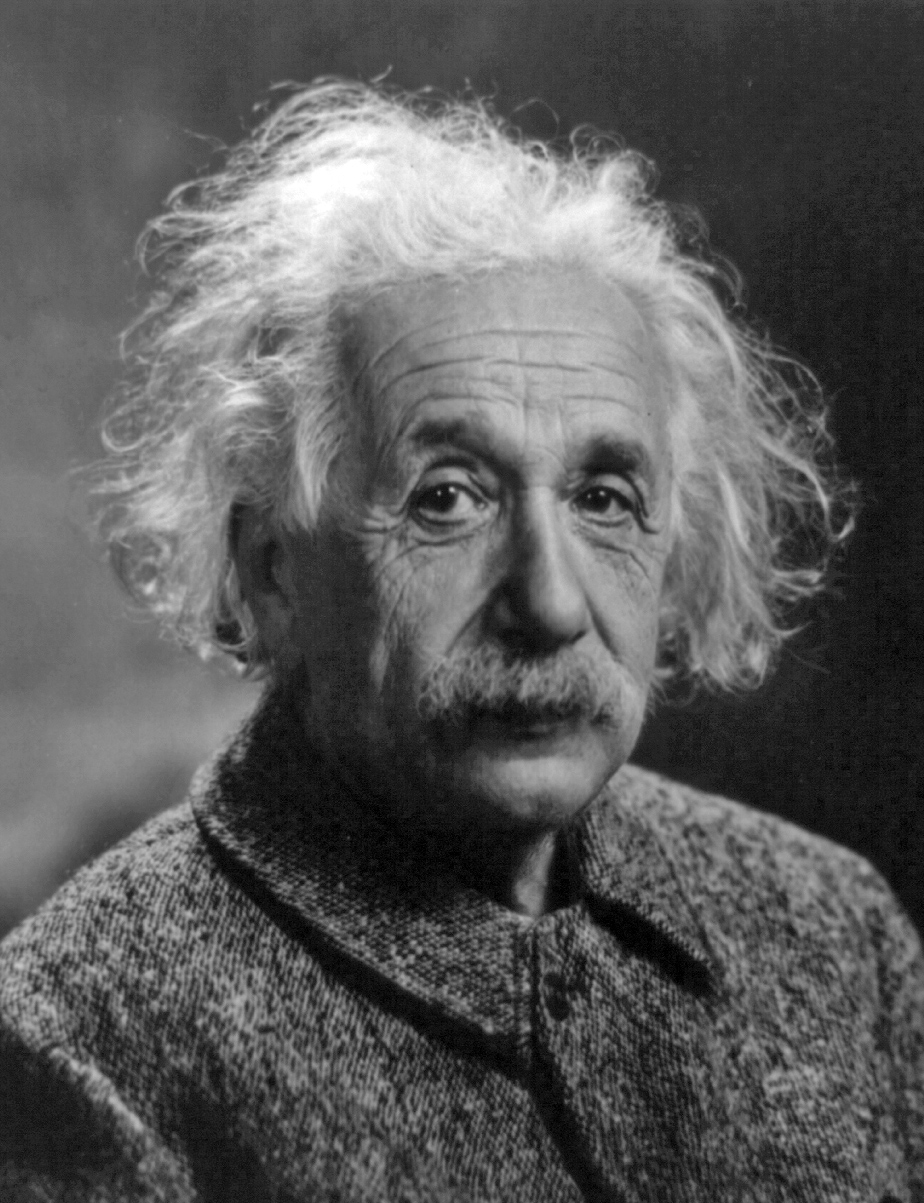
\includegraphics[height=35mm]{mypicture}}
\newcommand{\Photo}{}

\begin{document}
\linenumbers

\vspace*{4cm}
\title{ATLAS Higgs Physics Results}

\author{ Kurt Brendlinger, on behalf of the ATLAS Collaboration }

\address{~\\DESY, Notkestra\ss e 85,\\ 22607 Hamburg, Germany}

\maketitle\abstracts{
The Large Hadron Collider and the ATLAS Detector.
}

\section{Introduction}

The Large Hadron Collider (LHC) \cite{Evans:2008zzb} and the ATLAS Detector \cite{PERF-2007-01}.

Citations:
The ATLAS Detector \cite{PERF-2007-01}
Higgs decaying to $b\bar b$ \cite{HIGG-2018-50}
VBF $H{\rightarrow}WW$ \cite{HIGG-2017-14}
ttH diphoton \cite{ATLAS-CONF-2019-004}
Hbb and VH observation \cite{HIGG-2018-04}.

\section{Measurement of the $VH$ production mode in the $b\bar b$ decay channel}\label{sec:vh_bb}

\begin{figure}[!htbp]
\centering
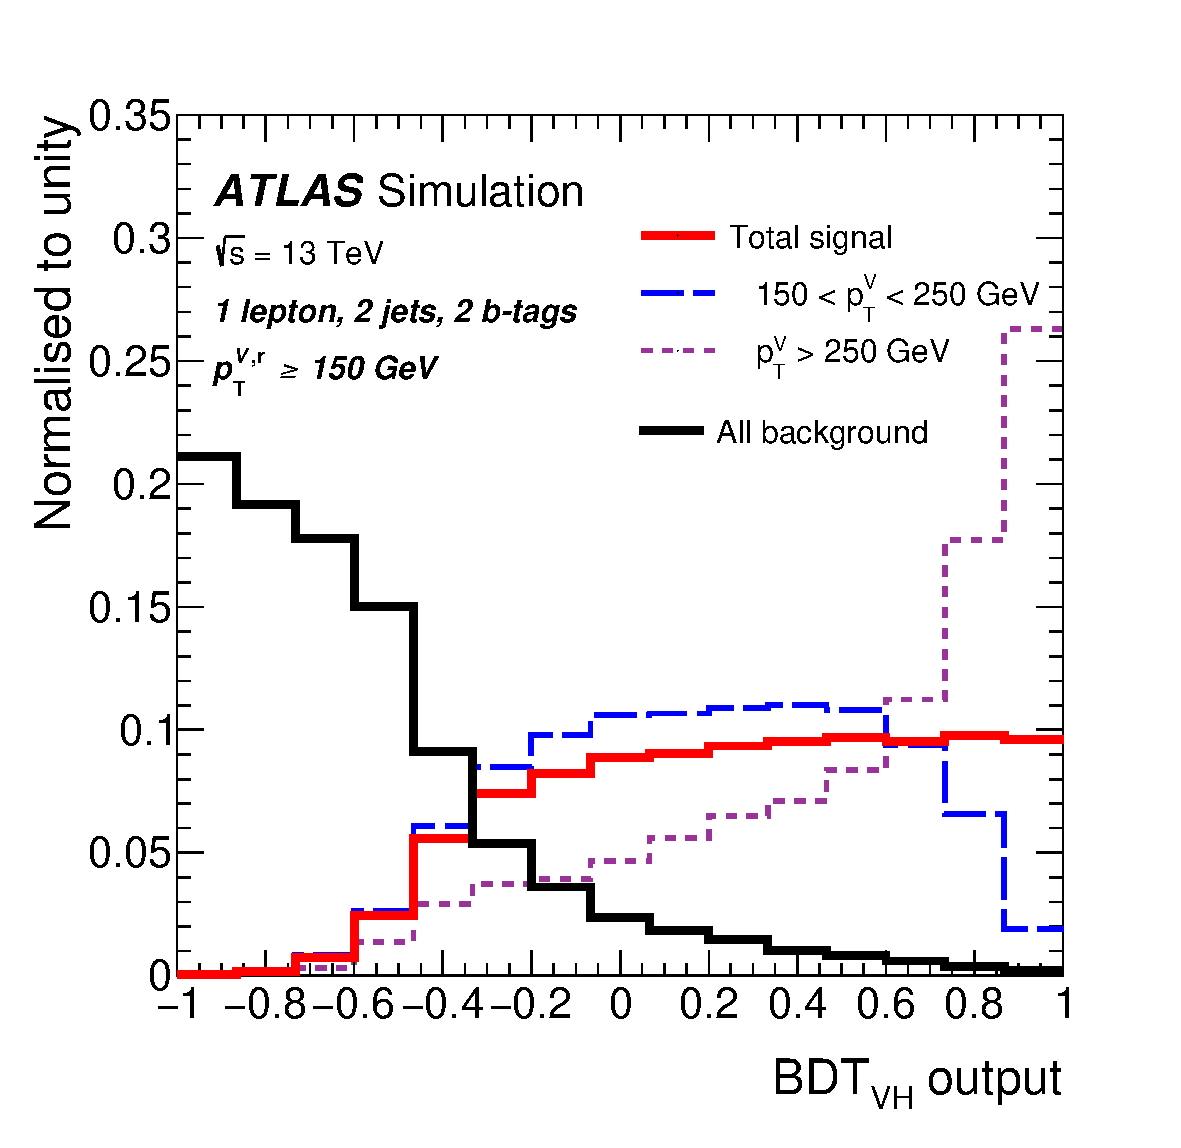
\includegraphics[width=0.425\linewidth]{figures/HIGG-2018-50/fig_01_v1.pdf}
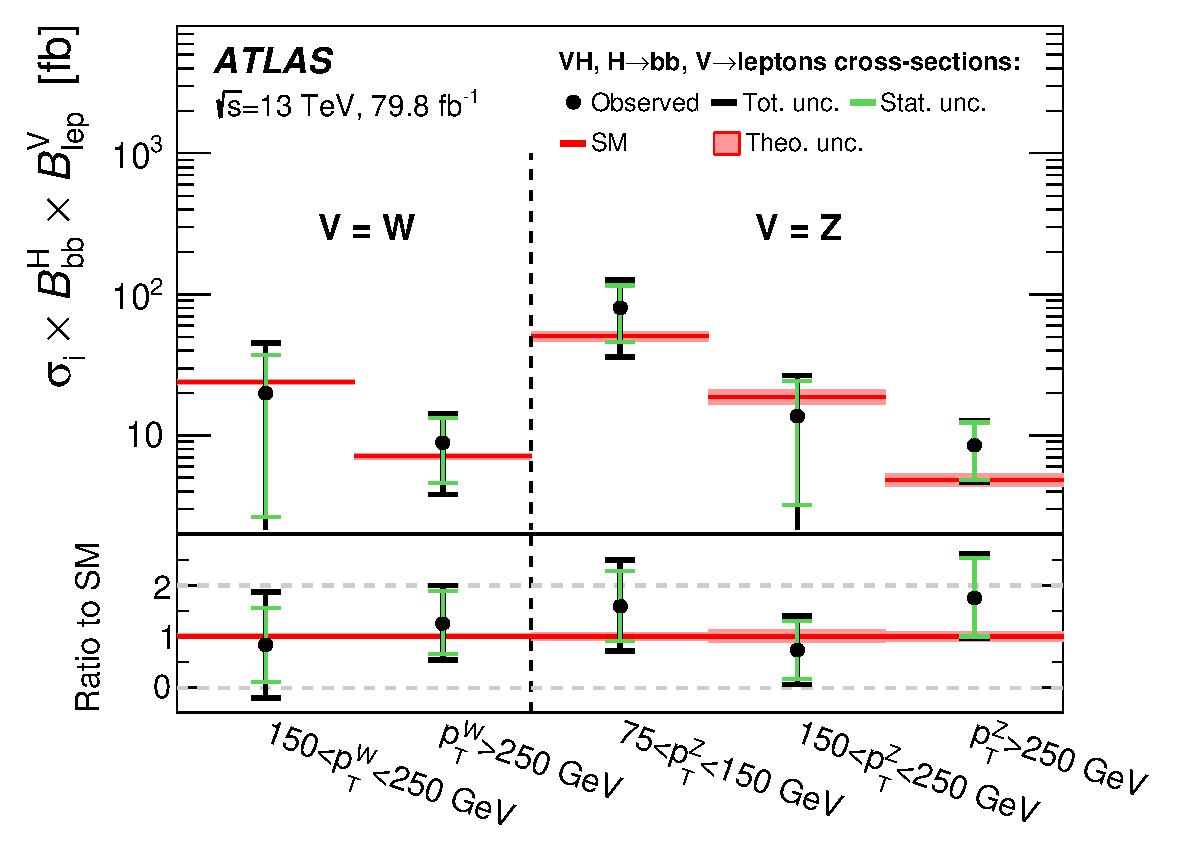
\includegraphics[width=0.565\linewidth]{figures/HIGG-2018-50/fig_03.pdf}
\caption{
  Left: the BDT. Right: The results.
}
\label{fig:vh_bb}
\end{figure}

\section{Measurement of Higgs production in association with a $t\bar t$ pair in the diphoton decay channel}\label{sec:ttH_yy}

\begin{figure}[!htbp]
\centering
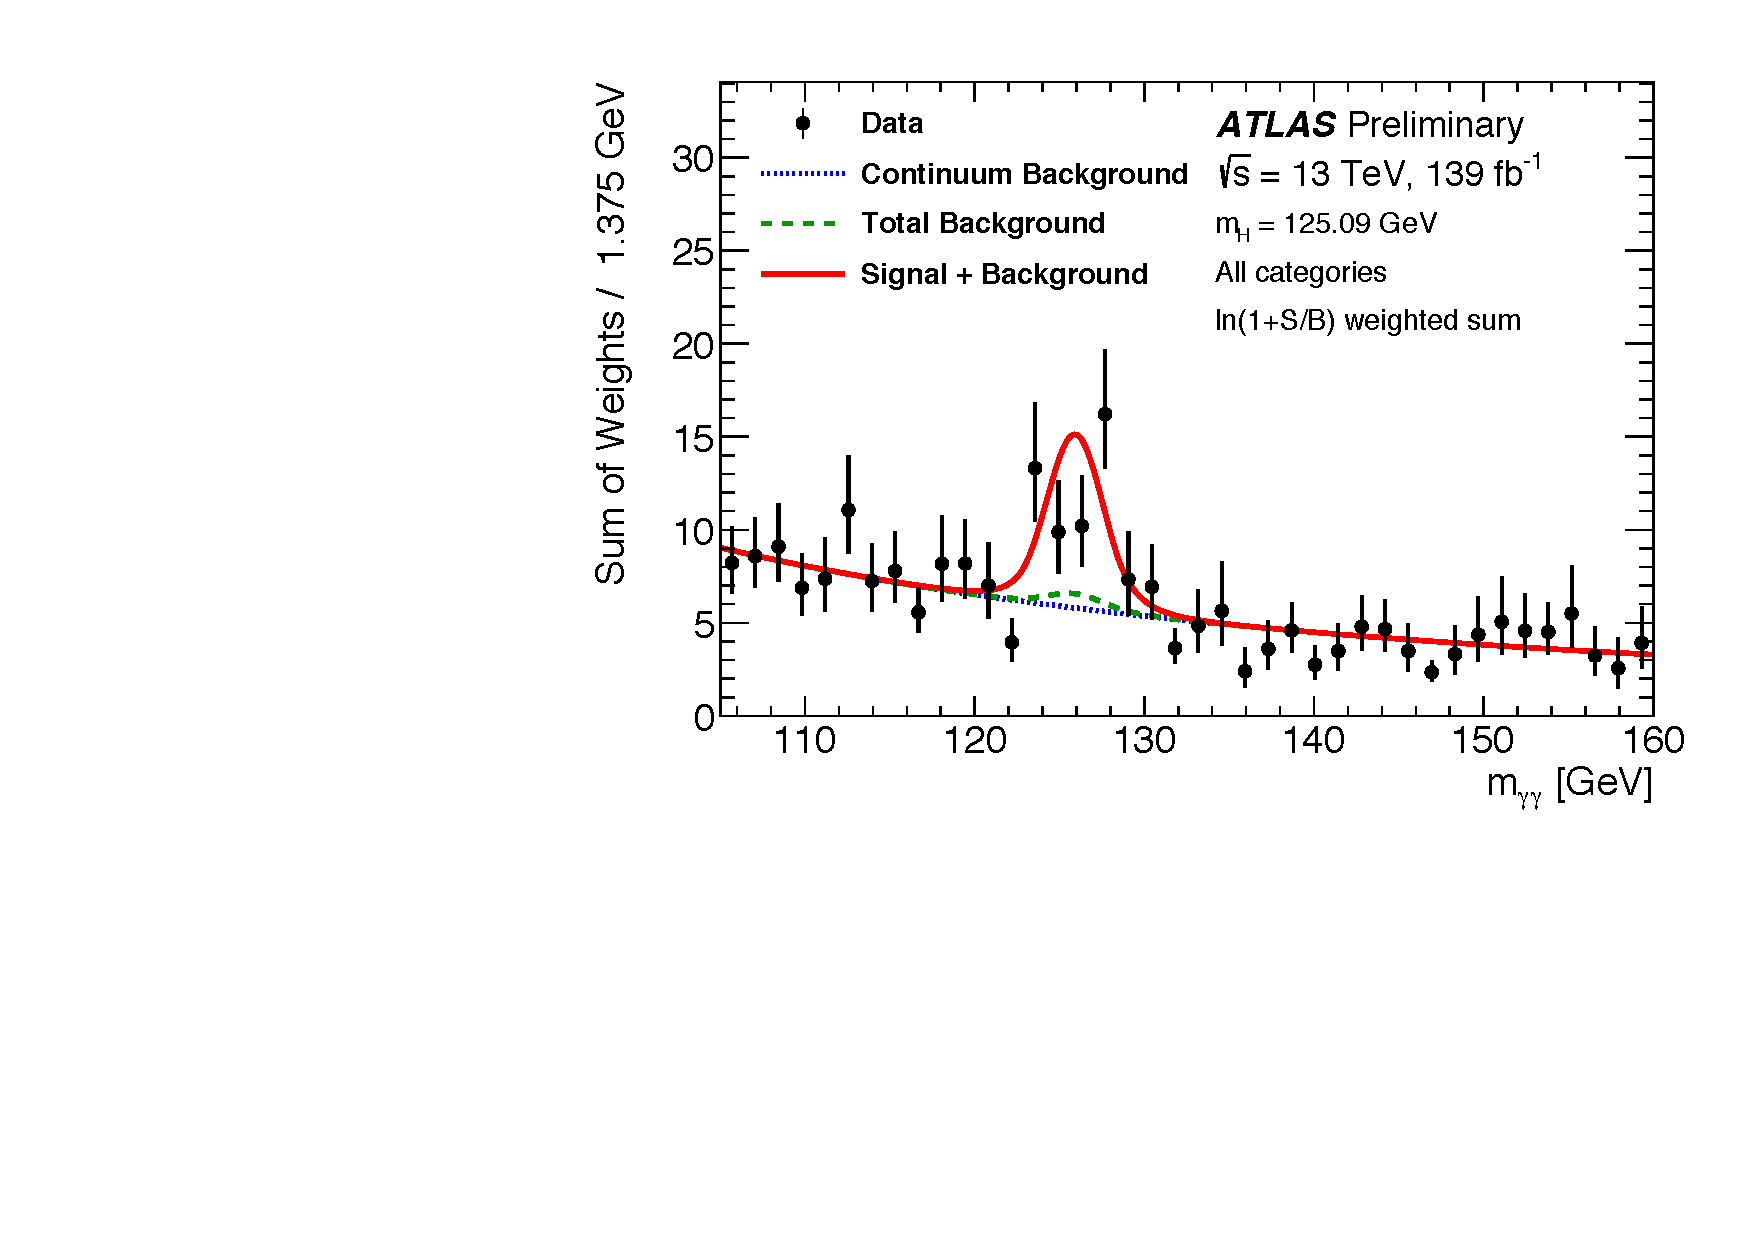
\includegraphics[width=0.525\linewidth]{figures/ATLAS-CONF-2019-004/fig_05_v1.pdf}
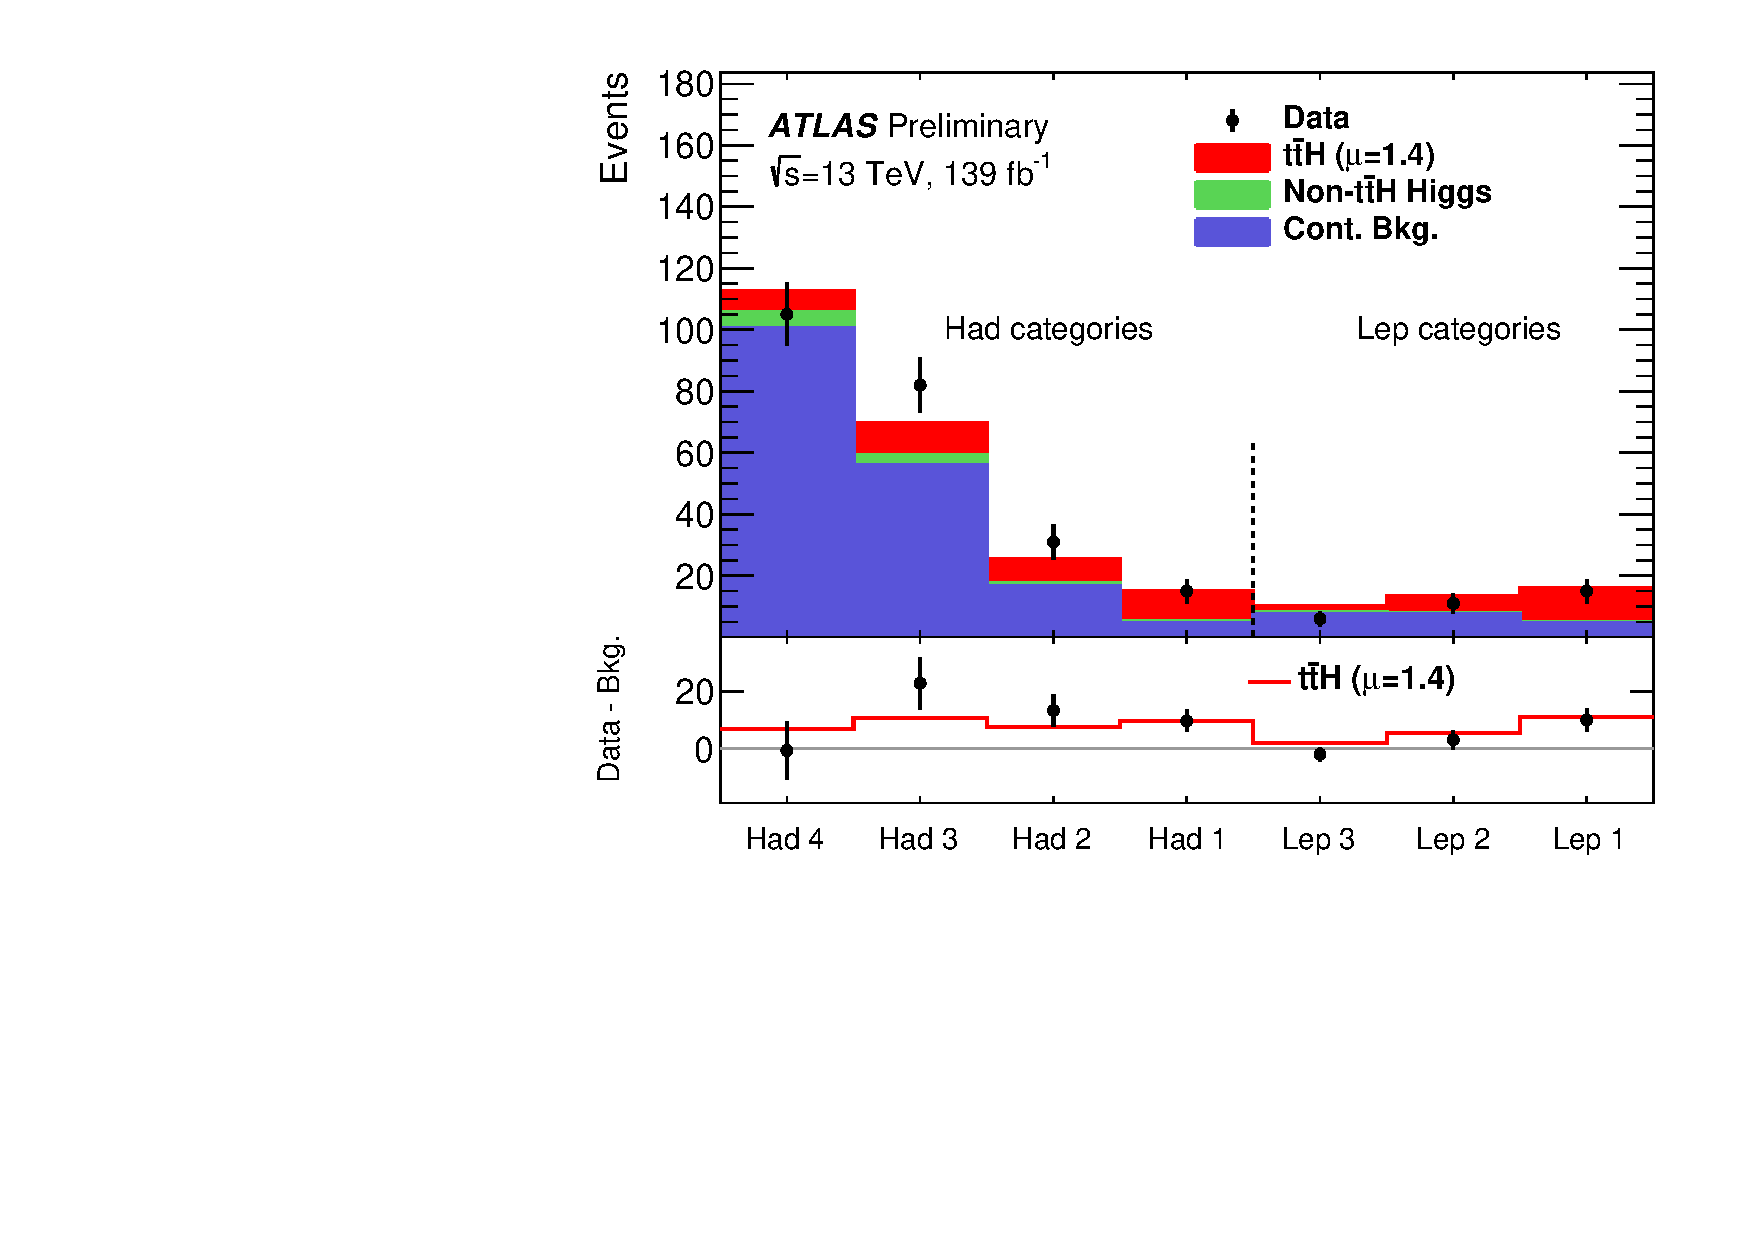
\includegraphics[width=0.465\linewidth]{figures/ATLAS-CONF-2019-004/fig_08.pdf}
\caption{
  ttH stuff.
}
\label{fig:vh_bb}
\end{figure}

\section{Measurement of the $VH$ production mode in the $WW$ decay channel} \label{sec:vh_ww}

Using 36.1~fb$^{-1}$.

\begin{figure}[!htbp]
\centering
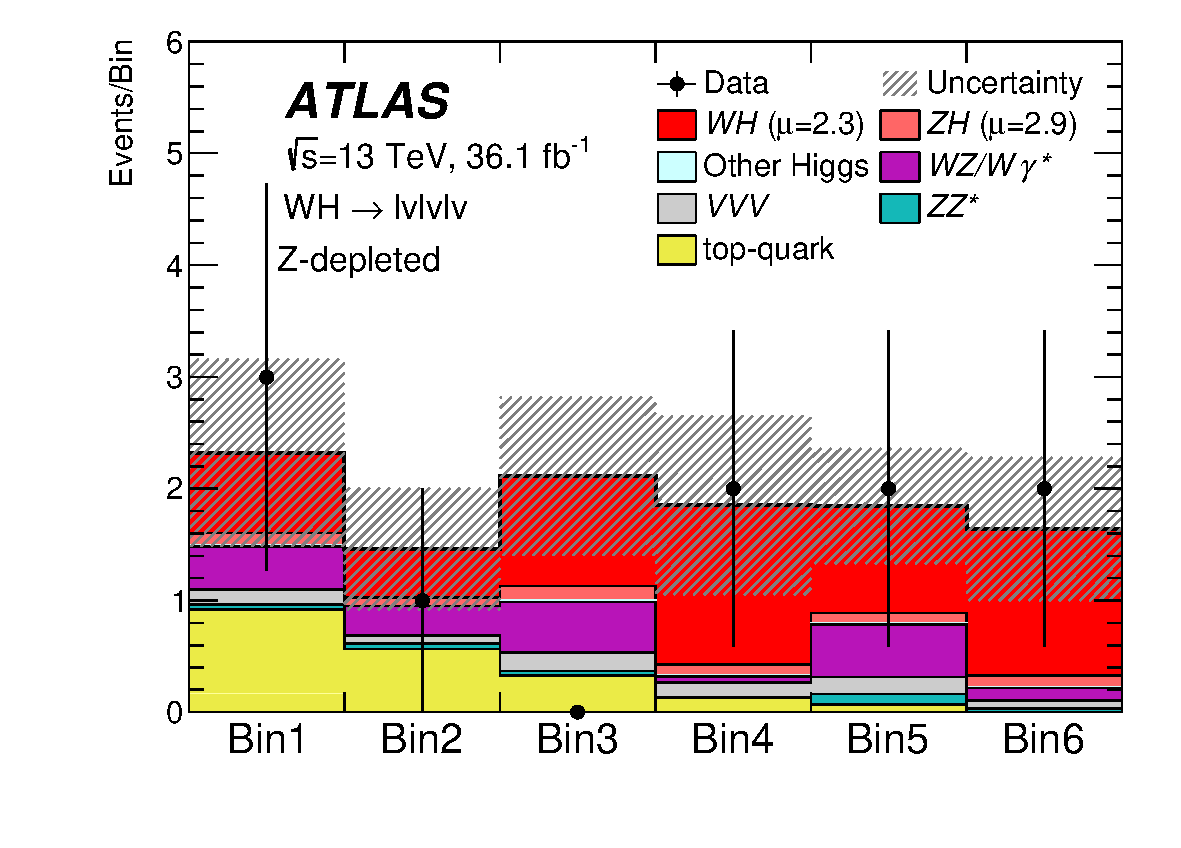
\includegraphics[width=0.55\linewidth]{figures/HIGG-2017-14/fig_06b.pdf}
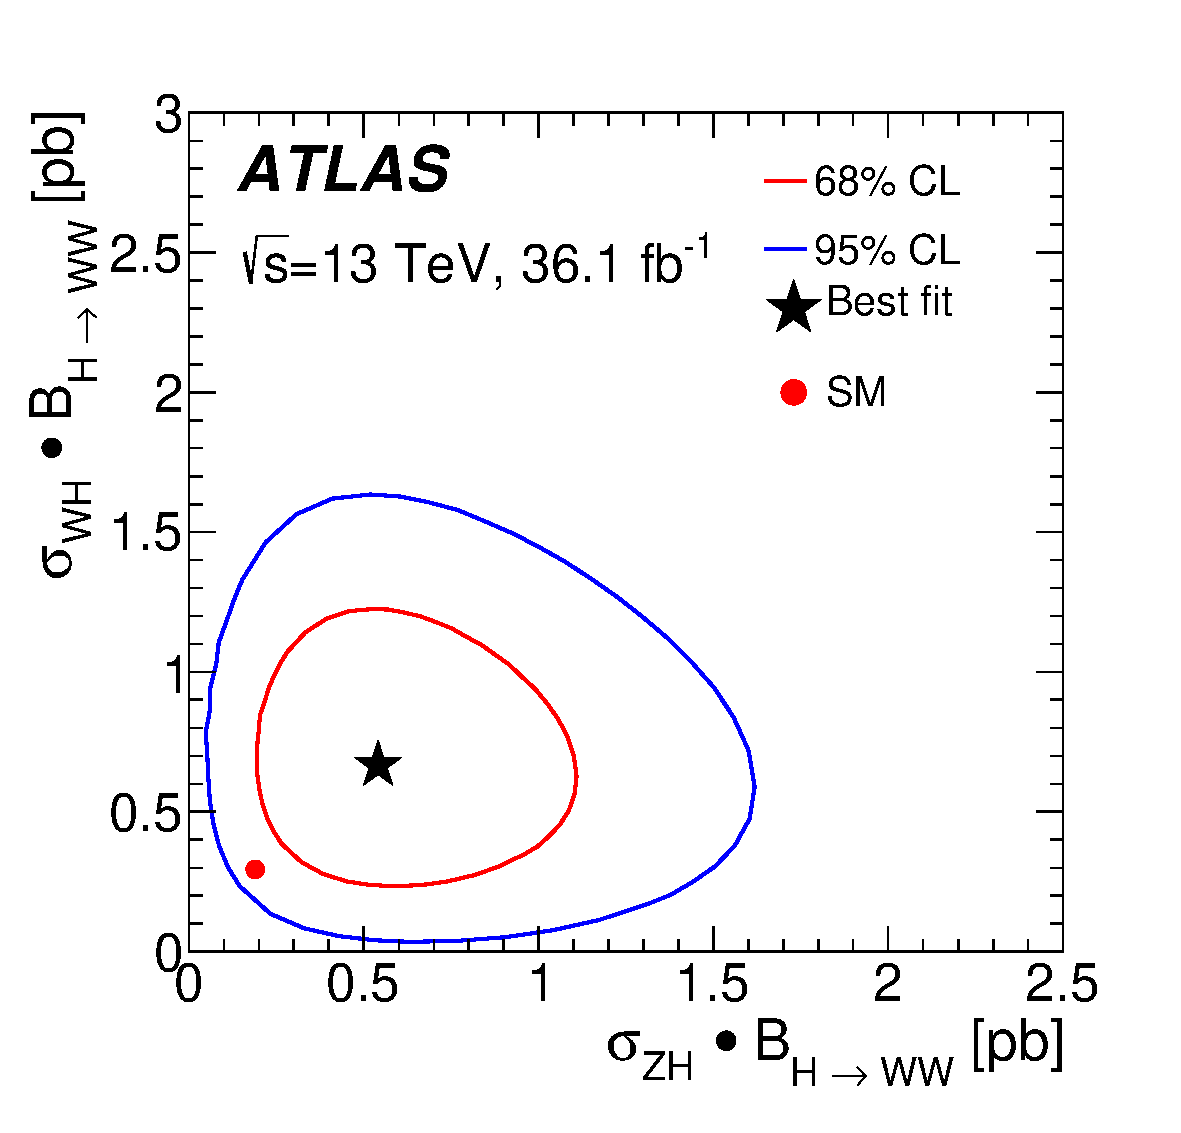
\includegraphics[width=0.44\linewidth]{figures/HIGG-2017-14/fig_08.pdf}
\caption{
  WW stuff.
}
\label{fig:vh_bb}
\end{figure}

\section{Limits on the Higgs Self Coupling} \label{sec:hh}

The limits are presented.

\section{Summary}

The Large Hadron Collider (LHC) \cite{Evans:2008zzb} and the ATLAS Detector.

% ATLAS-required copyright
% Authors should try to find a place that is not too obtrusive for this statement e.g. as footnote
% on the first page or just before the references
Copyright 2019 CERN for the benefit of the ATLAS Collaboration. CC-BY-4.0 license.

\section*{References}

\bibliography{brendlinger}

\end{document}

%%%%%%%%%%%%%%%%%%%%%%
% End of moriond.tex  %
%%%%%%%%%%%%%%%%%%%%%%
